\documentclass{beamer}
%\documentclass[handout]{beamer}  % for handout

%\usepackage{pgfpages}  % for handout
%\pgfpagesuselayout{4 on 1}[letterpaper,landscape,border shrink=5mm] % for handout
%\setbeamertemplate{footline}[frame number] % for handout

\usefonttheme[onlymath]{serif}  % use "article"-style math font

\usepackage[utf8]{inputenc} % allow utf-8 input
%\usepackage[T1]{fontenc}    % use 8-bit T1 fonts
\usepackage{hyperref}       % hyperlinks
\usepackage{url}            % simple URL typesetting
\usepackage{booktabs}       % professional-quality tables
\usepackage{amsmath}
\usepackage{amssymb}
\usepackage{amsthm}
\usepackage{amsfonts}       % blackboard math symbols
\usepackage{mathtools}
\usepackage{nicefrac}       % compact symbols for 1/2, etc.
\usepackage{microtype}      % microtypography
\usepackage{algorithm}
\usepackage{algpseudocode}
\usepackage{graphicx}
\usepackage{float}
\usepackage{caption}
\usepackage{tikz}

\usetikzlibrary{bayesnet,positioning}

\newcommand{\len}{\mathop{\text{len}}}
\newcommand{\nth}{^{\text{th}}}
\newcommand{\customSectionFrame}[1]{%
  \begin{frame}[c]{ } %
  \Large
  \color[rgb]{0,0,0.6}
  \centering %
  #1 %
  \end{frame}%
  }

\setbeamertemplate{blocks}[default]
\setbeamertemplate{navigation symbols}{}  % Omit navigation buttons
\setbeamertemplate{bibliography item}{\insertbiblabel}

\title{Hierarchical Topic Models}
\author{Andrew Leverentz \\[1em] %
    { \small %
    \emph{Research Examination, Fall Quarter 2017} \\ %
    \emph{UC San Diego, Dept.\ of Computer Science and Engineering}}}
\date{}
% TODO: \titlegraphic{\includegraphics[width=0.3\textwidth]{figures/some-figure.png}}

\begin{document}

\begin{frame}
\titlepage
\end{frame}

\begin{frame}
\frametitle{Context}
\begin{itemize}[<+->]
\item Internet and digital archives $\rightarrow$ large collections of text data
\item How can we navigate these collections efficiently?
\item Typical task: find sets of documents that share the same topic or subject matter
\item Ambiguities of natural language $\rightarrow$ superficial attributes of documents aren't enough
    \begin{itemize}[<+->]
    \item \emph{Synonymy}: Many words, same meaning
    \item \emph{Polysemy}: One word, many meanings (depending on context)
    \end{itemize}
\item We need a notion of \emph{latent semantics}, or underlying meaning
\end{itemize}
\end{frame}

\begin{frame}
\frametitle{Goals}
\begin{itemize}[<+->]
\item General approach: documents are mixtures of topics, which are distributions over the vocabulary
\item Probability provides a natural framework for this
\item Topics can exist at different levels of abstraction (e.g., \emph{baseball} and \emph{basketball} are distinct subtopics under \emph{sports})
\item Can we learn a hierarchy of topics based on a particular corpus?
\item Similar to the Dewey Decimal System or Library of Congress Classification
\end{itemize}
\end{frame}

\begin{frame}
\frametitle{Latent Semantic Analysis: A Non-Probabilistic Precursor}
\begin{itemize}[<+->]
\item Compute matrix of word frequencies:
\[ M_{i,j} = \text{number of times the $i\nth$ word appears in document $j$} \]
\item Optionally, transform via per-term and per-document statistics
\[ X_{i,j} = f(M_{i,j}, M_{i,1:D}, M_{1:N,j}) \]
\item Compute singular-value decomposition (SVD) of this matrix
\[ X = U \Sigma V^\top \]
\item Low-rank truncation represents documents and terms as low-dimensional \emph{latent semantic vectors}
\item Similarity between documents $=$ normalized dot product of latent semantic vectors
\end{itemize}
\end{frame}

\begin{frame}
\frametitle{Probabilistic Latent Semantic Analysis}
\begin{itemize}[<+->]
\item Idea: frequencies of words in documents determined by probabilities
\item There are $K$ latent topics, and each $\theta_k$ is a distribution over words in the vocabulary
\item For document $d$, the vector $\phi_d$ is a distribution over topics
\item For the $n\nth$ word in document $d$:
\begin{alignat*}{2}
\text{Select a topic:}&\qquad& z_{d,n} &\sim \text{Categorical}(\phi_d) \\
\text{Select a word:}&\qquad& t_{d,n} &\sim \text{Categorical}(\theta_{z_{d,n}})
\end{alignat*}
\onslide<.->
\begin{center}
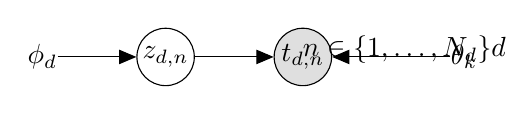
\begin{tikzpicture}
\node[obs] (t) {$t_{d,n}$};
\node[const, right=1.5cm of t] (theta) {$\theta_k$};
\node[latent, left=of t] (z) {$z_{d,n}$};
\node[const, left=of z] (phi) {$\phi_d$};

\edge{phi}{z};
\edge{theta}{t};
\edge{z}{t};

\centeredPlate{word-plate}{(t)(z)}{$n \in \{1, \ldots, N_d\}$};
\centeredPlate{doc-plate}{(word-plate)(phi)}{$d \in \{1, \ldots, D\}$};
\centeredPlate{topic-plate}{(theta)}{$k \in \{1, \ldots, K\}$};
\end{tikzpicture}
\end{center}
\end{itemize}

\begin{itemize}[<+->]
\item Infer values of $\theta_k$, $\phi_d$ using maximum likelihood
\end{itemize}
\end{frame}

\begin{frame}
\frametitle{Latent Dirichlet Allocation}
\begin{itemize}[<+->]
\item Extension to PLSA: assume topic mixtures $\phi_d$ and topic vectors $\theta_k$ are drawn from Dirichlet distributions
\item Dirichlet is a distribution over discrete probability distributions; density over simplex:
\[ \text{Dirichlet}(\vec x \mid \vec \alpha) \propto \prod_{k=1}^{\len(\vec\alpha)} x_i^{\alpha_i - 1} \]
\item Dirichlet distribution acts as a \emph{regularizer}, reduces overfitting
\item Allows Bayesian posterior inference
\end{itemize}
\end{frame}

\begin{frame}
\frametitle{Latent Dirichlet Allocation: The Model}
\begin{alignat*}{2}
\theta_k &\sim \text{Dirichlet}(\alpha) &\qquad&\text{for each topic $k$} \\
\phi_d &\sim \text{Dirichlet}(\beta) &\qquad&\text{for each document $d$} \\
z_{d,n} &\sim \text{Categorical}(\phi_d) &\qquad&\text{for the $n\nth$ word in document $d$} \\
t_{d,n} &\sim \text{Categorical}(\theta_{z_{d,n}}) &\qquad&\text{for the $n\nth$ word in document $d$}
\end{alignat*}

\begin{center}
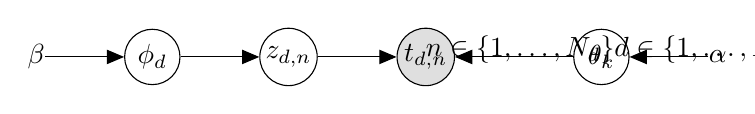
\begin{tikzpicture}
\node[obs] (t) {$t_{d,n}$};
\node[latent, right=1.5cm of t] (theta) {$\theta_k$};
\node[latent, left=of t] (z) {$z_{d,n}$};
\node[latent, left=of z] (phi) {$\phi_d$};
\node[const, right=of theta] (alpha) {$\alpha$};
\node[const, left=of phi] (beta) {$\beta$};

\edge{alpha}{theta};
\edge{phi}{z};
\edge{beta}{phi};
\edge{theta}{t};
\edge{z}{t};

\centeredPlate{word-plate}{(t)(z)}{$n \in \{1, \ldots, N_d\}$};
\centeredPlate{doc-plate}{(word-plate)(phi)}{$d \in \{1, \ldots, D\}$};
\centeredPlate{topic-plate}{(theta)}{$k \in \{1, \ldots, K\}$};
\end{tikzpicture}
\end{center}
\end{frame}

%%%%%%%%%%%%%

\customSectionFrame{Bayesian Inference Algorithms}

\begin{frame}
\frametitle{Posterior Inference}
\begin{itemize}[<+->]
\item Latent-variable models contain \emph{observed} and \emph{latent} random variables
\item Model specifies:
    \begin{itemize}
    \item<.-> \emph{Likelihood}: $p(\text{data} \mid \text{latent variables}, \text{fixed parameters})$
    \item<+-> \emph{Prior}: $p(\text{latent variables} \mid \text{fixed parameters})$
    \end{itemize}
\item Goal: try to estimate the \emph{posterior} via Bayes' rule
\begin{align*}
\MoveEqLeft
p(\text{latent variables} \mid \text{data}, \text{fixed parameters}) \\
&=
\frac{\text{Likelihood} \times \text{Prior}}
     {p(\text{data} \mid \text{fixed parameters})}
\end{align*}
\item Denominator: marginalization is often intractable
\item Need approximate inference methods
\end{itemize}
\end{frame}

\begin{frame}
\frametitle{Gibbs Sampling}
\begin{itemize}[<+->]
\item Markov Chain Monte Carlo (MCMC) method
    \begin{itemize}[<+->]
    \item \emph{Monte Carlo}: Estimate a quantity by drawing samples from a random distribution
    \item \emph{Markov Chain}: Find stationary distribution of a stochastic process where update rules depend only on previous state
    \end{itemize}
\item State vector $\vec z$; each component corresponds to a latent variable
\item Repeatedly update $\vec z$ by iterating through random variables, updating $z_k$ by sampling from its \emph{complete conditional}:
\[ p(z_k \mid \vec z_{-k}, \vec x) \]
Here, $\vec z_{-k}$ denotes all components of $\vec z$ except $z_k$
\item The distribution of the samples $\vec z$ approaches the true posterior $p(\vec z \mid \vec x)$
\end{itemize}
\end{frame}

\begin{frame}
\frametitle{Collapsed Gibbs Sampling}
\begin{itemize}[<+->]
\item For some models, we can eliminate some latent variables by marginalization
\item For the remaining latent variables, we compute a modified form of the complete conditionas:
\[ p(z_k \mid \vec z_{\text{subset}-k}, \vec x) \]
\item Running Gibbs sampling based on these distributions yields an estimate for
\[ p(\vec z_{\text{subset}} \mid \vec x) \]
%\item Estimating the eliminated variables requires post-processing
\end{itemize}
\end{frame}

\begin{frame}
\frametitle{Variational Inference}
\begin{itemize}[<+->]
\item Approximation technique: select an approximating family of distributions and search for best approximation
\item Measure closeness using reversed Kullback-Leibler divergence
\item Mean-field approximation: consider parameterized functions which factor cleanly:
\[ q(\vec z) = \prod_k q_k(z_k; \nu_k) \]
\item Minimizing reversed KL corresponds to maximizing \emph{evidence lower bound} (ELBO):
\[ \text{ELBO} = E_q[\log p(\vec z, \vec x)] - E_q[\log q(\vec z)] \]
\end{itemize}
\end{frame}

\begin{frame}
\frametitle{Coordinate-Ascent Variational Inference}
\begin{itemize}[<+->]
\item Coordinate ascent: optimize one latent variable's parameters at a time
\item Works best for exponential-family models, where conditional distributions can be written as
\[ p(x \mid \theta) = h(x) \exp( \alert<.(1)>{\eta(\theta)} \cdot \alert<.(2)>{T(x)} - a(\theta)) \]
\onslide<+->{(\alert<.>{$\eta(\theta) =$ \emph{natural parameters}}, \alert<+>{$T(x) =$ \emph{sufficient statistics}})} \pause
\item For exponential-family models, the update rule for $z_k$ is
\[ \nu_k = E_q[\eta_k(\vec z_{-k}, \vec x)] \]
where $\eta_k$ denotes the natural parameters of the complete conditional of $z_k$
\end{itemize}
\end{frame}

\begin{frame}
\frametitle{Stochastic Variational Inference: Context}
\begin{itemize}[<+->]
\item Generic model with local (per-observation) and global variables:
\begin{center}
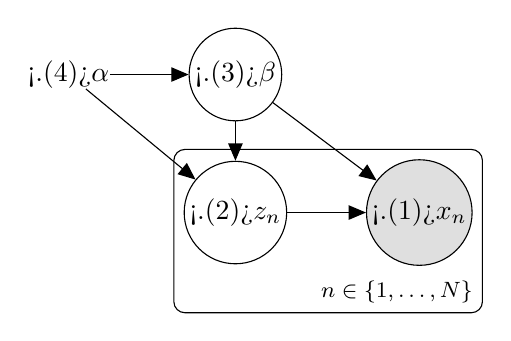
\begin{tikzpicture}
\node[obs] (x) {\alert<.(1)>{$x_n$}};
\node[latent, left=of x] (z) {\alert<.(2)>{$z_n$}};
\node[latent, above=0.5cm of z] (beta) {\alert<.(3)>{$\beta$}};
\node[const, left=of beta] (alpha) {\alert<.(4)>{$\alpha$}};

\edge{z}{x};
\edge{beta}{z};
\edge{beta}{x};
\edge{alpha}{beta};
\edge{alpha}{z};

\plate{obs-plat}{(x)(z)}{$n \in \{1, \ldots, N\}$};
\end{tikzpicture}
\end{center}
\onslide<+->{\alert<.>{$x_n$}: observed data} \\
\onslide<+->{\alert<.>{$z_n$}: local variables (one per observation)} \\
\onslide<+->{\alert<.>{$\beta$}: global variable (shared for all observations)} \\
\onslide<+->{\alert<.>{$\alpha$}: fixed parameters}
\item Complete conditional for local variables simplifies:
\[ p(z_n \mid \alpha, \beta, z_{-n}, x_{1:N}) = p(z_n \mid \alpha, \beta, x_n) \]
\item Complete conditional for global variable requires full dataset:
\[ p(\beta \mid \alpha, z_{1:N}, x_{1:N}) \]
\end{itemize}
\end{frame}

\begin{frame}
\frametitle{Stochastic Variational Inference: Natural Gradient}
\begin{itemize}[<+->]
\item Euclidean distance on variational parameters may not reflect ``true'' distance between distributions
\item Rather than standard gradient of the objective function ($\nabla \mathcal L$), use natural gradient $G^{-1} \nabla \mathcal L$
\item $G$ is a matrix (\emph{metric tensor}) that encodes local information about ``true'' distances
\item With a symmetric version of KL divergence and a model with exponential-family distributions, $G$ cancels cleanly:
\[ G^{-1} \nabla \mathcal L = E_q[\eta] - \nu \]
where $\nu$ is the current value of the local variational params
\item For local variables, the update rule is the same as in CAVI:
\[ \nu^{\text{local}} = E_q[\eta^{\text{local}}] \]
\end{itemize}
\end{frame}

\begin{frame}
\frametitle{Stochastic Variational Inference: Global Updates}
\begin{itemize}[<+->]
\item For global variables, repeatedly draw \emph{mini-batches} $b$ containing $S$ observations
\item Compute an \emph{unbiased estimate} of the natural gradient $G^{-1} \nabla \mathcal L$ for each batch:
\[ \mu = E_q[\alert<.(1)>{\eta^{\text{global}}_b}] - \nu^{\text{global}} \]
\onslide<+->{Here, \alert<.>{$\eta^{\text{global}}_b$} denotes the natural parameters of the complete conditional of the global variable, but with the true dataset replaced by $N / S$ copies of the mini-batch $b$}
\item Update according to a decaying schedule of step sizes $\rho_t$:
\begin{align*}
\nu^{\text{global}}
&\gets \nu^{\text{global}} + \rho_t \, \mu \\
\onslide<+->{ &= (1-{\rho_t}) \nu^{\text{global}} + {\rho_t} \, E_q[\eta^{\text{global}}_b] }
\end{align*}
%\onslide<+->{Here, \alert<.>{$\rho_t$} should satisfy $\sum_{t\geq1} \rho_t = \infty$ and $\sum_{t\geq1} \rho_t^2 < \infty$}
\end{itemize}
\end{frame}

%%%%%%%%%%%%%

\customSectionFrame{Learning Topic Hierarchies}

\begin{frame}
\frametitle{Topic Modeling with Hierarchies}
\begin{itemize}[<+->]
\item Goal: extend LDA model so that:
    \begin{itemize}[<+->]
    \item Topics are arranged in a tree \\ (root $\rightarrow$ abstract; leaves $\rightarrow$ concrete)
    \item The size and structure of the tree can be determined in a data-driven way
    \end{itemize}
\item Documents can combine topics, but in a more constrained way
    \begin{itemize}
    \item If a document draws words from one node, then it should also be somewhat likely to draw words from ancestor nodes
    \end{itemize}
\item We'll discuss two main models:
    \begin{itemize}
    \item Nested Chinese Restaurant Process
    \item Nested Hierarchical Dirichlet Process
    \end{itemize}
\end{itemize}
\end{frame}

\begin{frame}
\frametitle{Nested Chinese Restaurant Process}
\begin{itemize}[<+->]
\item Idea: Each document samples a path from an infinite tree
\item Within each document, we can only select nodes (ie, topics) from the sampled path
\vspace{1em}
\item How to define distributions over paths in an infinite (or arbitrarily large) tree? \\
\onslide<+->{Nested Chinese Restaurant Process}
\item How to define distributions over arbitrarily large partitions? \\
\onslide<+->{Chinese Restaurant Process}
\end{itemize}
\end{frame}

\begin{frame}
\frametitle{Chinese Restaurant Process: Distribution Over Partitions}
\begin{itemize}[<+->]
\item Analogy: Sequence of customers entering a restaurant
\item Infinitely many tables, each with infinite capacity
\item First customer always sits at first table
\item When $n \geq 1$ customers have been seated, the next customer follows these rules:
    \begin{itemize}
    \item If the first $k$ tables are occupied, with the $i\nth$ table containing $m_i$ customers, sit at table $i$ with probability $\frac{m_i}{n+\alpha}$
    \item Sit at the next empty table with probability $\frac{\alpha}{n + \alpha}$
    \end{itemize}
\item Parameter $\alpha$: as $\alpha \to \infty$, number of occupied tables increases
\end{itemize}
\end{frame}

\begin{frame}
\frametitle{Dirichlet Process: Distribution Over Grouped Data}
\begin{itemize}[<+->]
\item TODO
\end{itemize}
\end{frame}

\begin{frame}
\frametitle{Nested CRP: Distribution Over Paths}
\begin{itemize}[<+->]
\item TODO
\end{itemize}
\end{frame}

\begin{frame}
\frametitle{NCRP Topic Model}
\begin{itemize}[<+->]
\item TODO
\end{itemize}
\end{frame}

\begin{frame}
\frametitle{Nested Hierarchical Dirichlet Process}
\begin{itemize}[<+->]
\item Idea: Global probability distribution over nodes, and each document samples a re-weighted version of that distribution
\end{itemize}
\end{frame}

%%%%%%%%%%%%%

\customSectionFrame{Thank You!}

{
\setbeamertemplate{frametitle continuation}{}
\setbeamerfont{bibliography item}{size=\footnotesize}
\setbeamerfont{bibliography entry author}{size=\footnotesize}
\setbeamerfont{bibliography entry title}{size=\footnotesize}
\setbeamerfont{bibliography entry location}{size=\footnotesize}
\setbeamerfont{bibliography entry note}{size=\footnotesize}
\begin{frame}[allowframebreaks]
\frametitle{References}
\nocite{*}
%\bibliographystyle{amsalpha}
%\bibliographystyle{plainnat}
\bibliographystyle{plain}
\bibliography{../bibliography}
\end{frame}
}

\end{document}
